\documentclass{beamer}\usepackage[]{graphicx}\usepackage[]{color}
% maxwidth is the original width if it is less than linewidth
% otherwise use linewidth (to make sure the graphics do not exceed the margin)
\makeatletter
\def\maxwidth{ %
  \ifdim\Gin@nat@width>\linewidth
    \linewidth
  \else
    \Gin@nat@width
  \fi
}
\makeatother

\definecolor{fgcolor}{rgb}{0.345, 0.345, 0.345}
\makeatletter
\@ifundefined{AddToHook}{}{\AddToHook{package/xcolor/after}{\definecolor{fgcolor}{rgb}{0.345, 0.345, 0.345}}}
\makeatother
\newcommand{\hlnum}[1]{\textcolor[rgb]{0.686,0.059,0.569}{#1}}%
\newcommand{\hlstr}[1]{\textcolor[rgb]{0.192,0.494,0.8}{#1}}%
\newcommand{\hlcom}[1]{\textcolor[rgb]{0.678,0.584,0.686}{\textit{#1}}}%
\newcommand{\hlopt}[1]{\textcolor[rgb]{0,0,0}{#1}}%
\newcommand{\hlstd}[1]{\textcolor[rgb]{0.345,0.345,0.345}{#1}}%
\newcommand{\hlkwa}[1]{\textcolor[rgb]{0.161,0.373,0.58}{\textbf{#1}}}%
\newcommand{\hlkwb}[1]{\textcolor[rgb]{0.69,0.353,0.396}{#1}}%
\newcommand{\hlkwc}[1]{\textcolor[rgb]{0.333,0.667,0.333}{#1}}%
\newcommand{\hlkwd}[1]{\textcolor[rgb]{0.737,0.353,0.396}{\textbf{#1}}}%
\let\hlipl\hlkwb

\usepackage{framed}
\makeatletter
\newenvironment{kframe}{%
 \def\at@end@of@kframe{}%
 \ifinner\ifhmode%
  \def\at@end@of@kframe{\end{minipage}}%
  \begin{minipage}{\columnwidth}%
 \fi\fi%
 \def\FrameCommand##1{\hskip\@totalleftmargin \hskip-\fboxsep
 \colorbox{shadecolor}{##1}\hskip-\fboxsep
     % There is no \\@totalrightmargin, so:
     \hskip-\linewidth \hskip-\@totalleftmargin \hskip\columnwidth}%
 \MakeFramed {\advance\hsize-\width
   \@totalleftmargin\z@ \linewidth\hsize
   \@setminipage}}%
 {\par\unskip\endMakeFramed%
 \at@end@of@kframe}
\makeatother

\definecolor{shadecolor}{rgb}{.97, .97, .97}
\definecolor{messagecolor}{rgb}{0, 0, 0}
\definecolor{warningcolor}{rgb}{1, 0, 1}
\definecolor{errorcolor}{rgb}{1, 0, 0}
\makeatletter
\@ifundefined{AddToHook}{}{\AddToHook{package/xcolor/after}{
\definecolor{shadecolor}{rgb}{.97, .97, .97}
\definecolor{messagecolor}{rgb}{0, 0, 0}
\definecolor{warningcolor}{rgb}{1, 0, 1}
\definecolor{errorcolor}{rgb}{1, 0, 0}
}}
\makeatother
\newenvironment{knitrout}{}{} % an empty environment to be redefined in TeX

\usepackage{alltt}					% Document class

\mode<presentation>
  {
    \usetheme{default}                    % Set theme
    \usecolortheme{default}               % Set colors
    \usefonttheme{default}                % Set font theme
    \setbeamertemplate{caption}[numbered] % Set caption to be numbered
  }

\usepackage{graphicx}  % For including figures
\usepackage{booktabs}  % For table rules
\usepackage{hyperref}  % For cross-referencing

\title{Introduction}  % Presentation title
\author{John Mensah}                              % Presentation author
\institute{University of Nebraska-Lincoln}                  % Author affiliation
\date{\today}                                    % Today's date

% This creates a bibliography file with the same name as the main file.
% Mostly, it allows us to have only one text file to lug around.
\IfFileExists{upquote.sty}{\usepackage{upquote}}{}
\begin{document}

% Title page
% This page includes the information defined earlier including
% title, author/s, affiliation/s and the date
\begin{frame}
\titlepage
\end{frame}

% Outline
% This page includes the outline (Table of content) of the presentation.
% All sections and subsections will appear in the outline by default.
\begin{frame}{Outline}
\tableofcontents
\end{frame}

% The following is the most frequently used slide types in beamer
% The slide structure is as follows:
  %
%\begin{frame}{<slide-title>}
%	<content>
  %\end{frame}

\section{Biography}

\begin{frame}{A brief introduction of Myself}
This is a bullet list of two points:
  \begin{itemize}
\item My name is John Mensah
\item My birthday is on March 23rd
\item I grew up in the Southern part of Ghana
\item I am studying a Ph.D. in Biological Science (with minor in Statistics) with a focus on Ecology, Evolution and Behavior
\item I hope to graduate in Spring 2025
\end{itemize}
\end{frame}

\section{Photo of favorite Animal}
\begin{frame}
\frametitle{Photos of my favorite Animal - Leopard}
\begin{center}
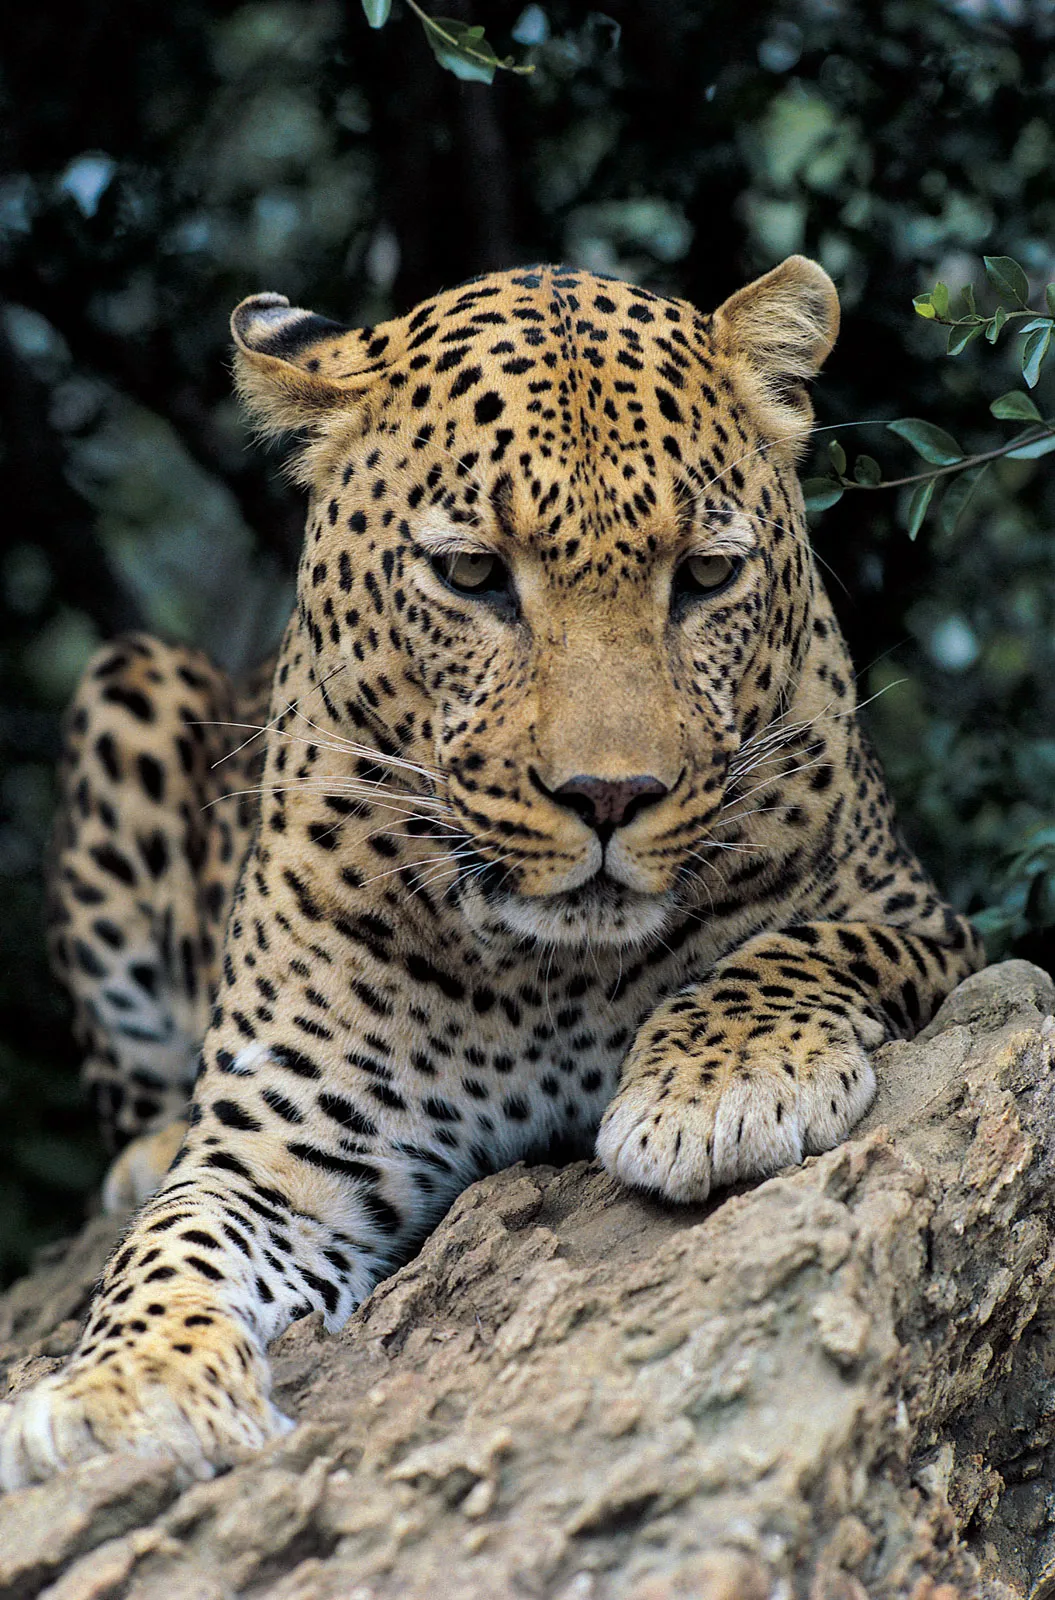
\includegraphics[width=.25\textwidth]{Leopard2.png}
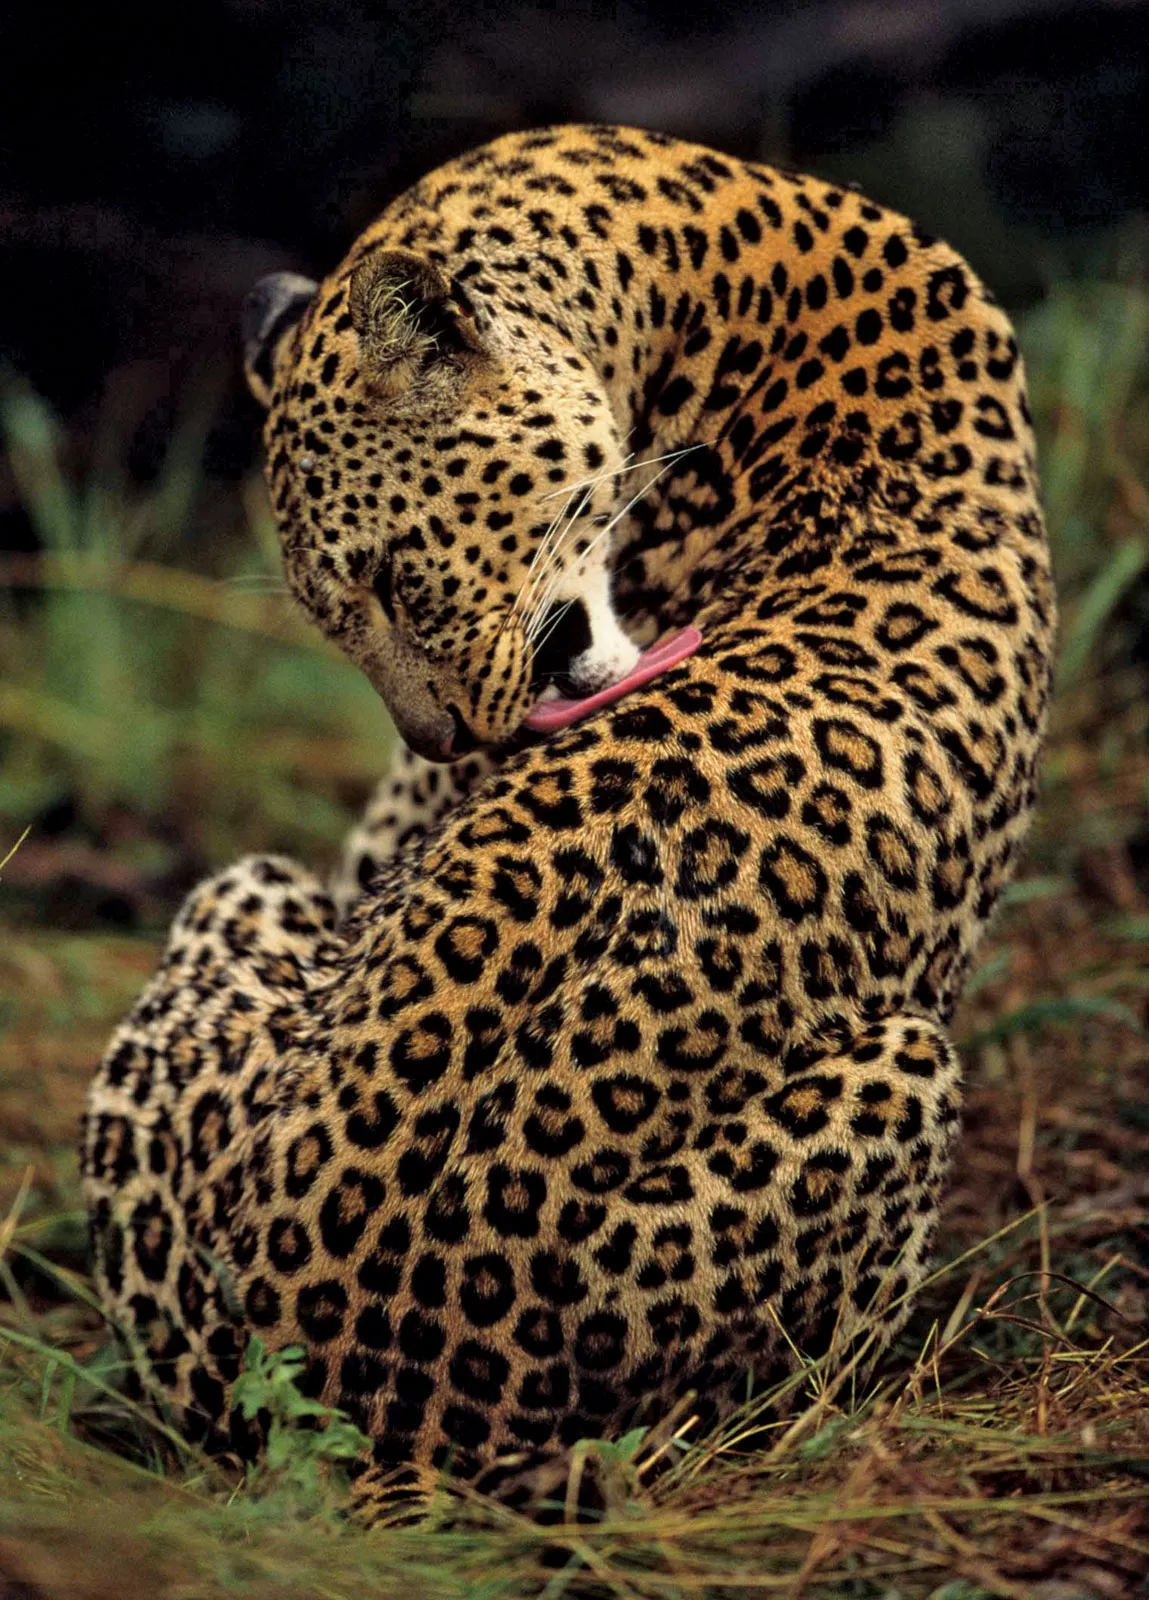
\includegraphics[width=.25\textwidth]{Leopard1.png}

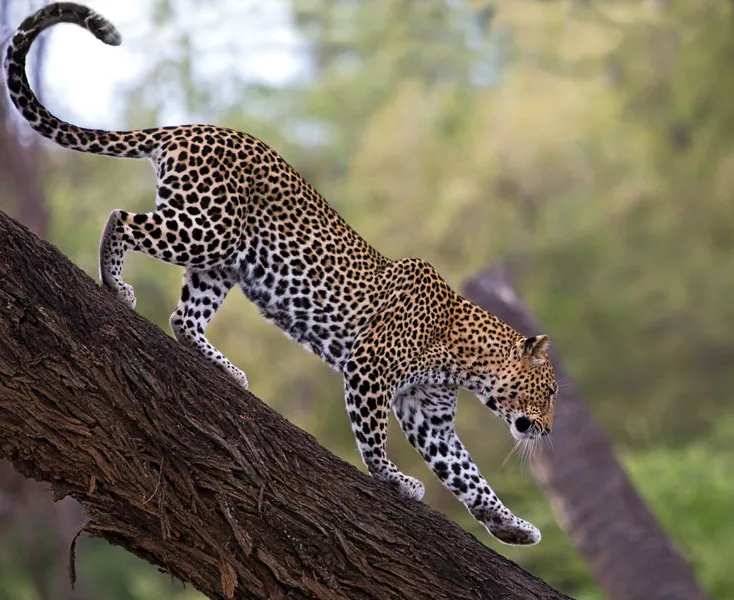
\includegraphics[width=.55\textwidth]{leopard.png}
\end{center}

\end{frame}





\section{Favorite plot}
\begin{frame}{Favorite plot}
\begin{knitrout}
\definecolor{shadecolor}{rgb}{0.969, 0.969, 0.969}\color{fgcolor}\begin{figure}
\includegraphics[width=\maxwidth]{figure/figure1-1} \caption[Change-point analysis of flowering pattern]{Change-point analysis of flowering pattern}\label{fig:figure1}
\end{figure}

\end{knitrout}
  \end{frame}

\section{Link to my CV}

\begin{frame}
A URL link to my CV: \url{https://github.com/JohnMensah50/JohnMensah50.github.io/blob/main/JohnMensah_CV.pdf}
\end{frame}

\end{document}




